\documentclass[UTF8]{ctexart} % 中文支持
\usepackage{xeCJK}

\setCJKmainfont{Noto Sans CJK SC}
\setmainfont{CMU Classical Serif}
% 设置字体

\setlength{\headheight}{20pt} % 主标题
\usepackage[a4paper, left=3.18cm, right=3.18cm, top=2.54cm, bottom=2.54em]{geometry} % a4纸张大小布局

\usepackage[colorlinks=true]{hyperref} %链接标注

% 网址换行
\usepackage{xurl}

% 基本信息
\newcommand{\titleValue}{在图片上快速编辑公式的编辑器设计}
\newcommand{\authorValue}{李沪纲}
\newcommand{\pagecounts}{10}

% 标题信息
\title{\titleValue}
\author{\authorValue}
\date{\today}

%页眉
\usepackage{fancyhdr}
\pagestyle{fancy}
\fancyhf{}
\lhead{\titleValue}
\rhead{ 第\thepage 页 \quad 共 \pagecounts 页 }
% 页眉标注主题和页码

\newcommand{\p}[1]{\paragraph{\mdseries{
    \indent #1
}}}

% 段落样式
\newcounter{refCounter}
\newcommand{\refTo}[1]{
    \label{reference-to-#1}\addtocounter{refCounter}{1}$^{
        \hyperref[reference-from-#1]{
            [\,\arabic{refCounter}\,]
        }
    }$
}
\newcommand{\refClear}{\setcounter{refCounter}{0}}
\newcommand{\refFrom}[1]{
    \noindent\label{reference-from-#1}\addtocounter{refCounter}{1}\hyperref[reference-to-#1]{$[\,\arabic{refCounter}\,]$}\,
}
% 文献引用

\usepackage{amsmath} % 数学

\usepackage{tikz} % 画图
\usetikzlibrary{positioning, shapes.geometric, graphs, quotes}

\usepackage{listings} % 代码块
\lstset{
    columns = fixed,
    numbers = left,
    frame = single,
    breaklines = true,
    showstringspaces = false,
    showtabs = true,
    tabsize = 4,
    aboveskip=4pt,
    belowskip=4pt,
    basicstyle=\ttfamily,
    backgroundcolor=\color[RGB]{255, 255, 255},
    keywordstyle=\color[RGB]{161, 84, 190},
    commentstyle=\color[RGB]{193, 190, 179},
    numberstyle=\color[RGB]{121, 185, 204},
    stringstyle=\color[RGB]{242, 192, 79},
    identifierstyle=\color[RGB]{86, 169, 218}
}
% 代码块样式

\usepackage{multirow}
% 表格

\renewcommand{\thefootnote}{\roman{footnote}}
% 脚注样式

\usepackage{xcolor}
% 颜色

\begin{document}

\maketitle
% 标题
\thispagestyle{empty}

\renewcommand{\abstractname}{\Large 摘要\\}
\begin{abstract}
    目前市场上的大多数图片编辑器都不支持公式编辑功能,而为广泛使用的 Microsoft Word 仅能在文档中添加公式,无法在图片上添加公式。学术界常用的排版系统 
    \LaTeX 
    也只能生成文档,但同样无法在现有的图片上编辑数学公式,这给用户带来了一定的不便。为了解决这一问题,本论文设计了一个能够快速在图片上编辑公式的编辑器,并提供了相关工程实现。
    \\
    \noindent{
        \textbf{
            关键词:
        }
        公式;公式编辑器;图片处理
    }
\end{abstract}
\thispagestyle{empty}

\tableofcontents
\thispagestyle{empty}
% 目录

\newpage
\setcounter{page}{1}
% 目录,摘要

\section{绪论}
\subsection[研究背景]{研究背景}
\p{
    如今,有许多工具能帮助人们在电脑上编辑公式。例如,Microsoft Word \refTo{microsoft-word-introduction}
    ,\LaTeX
    \refTo{latex-introduction}
    等。但是,这些工具都只能编辑或生成文档,不能很方便的对图片进行操作。到目前为止,在图片上编辑公式最方便的办法就是使用多数图片编辑器中自带的画笔,结合手写板进行手写,但是,手写板毕竟只是字迹,写出来的公式带有个人的笔风,并不像Word和\LaTeX
    所生成的那么标准,并且容易写错和被人误认。而且,没有手写板时,只用鼠标写出来的字迹不堪入目。
}

\subsection[研究目的与意义]{研究目的与意义}
\p{
    对此,我们意图发明一个能快速在图片上编辑公式的编辑器,能帮助广大教师学生更好的批改作业、分享题目思路解答,提高效率,节省时间。
}

\subsection[创新点]{创新点}
\p{
    在Microsoft Word中,编辑公式需要用鼠标去点击,虽说操作起来比较简单,上手难度低,但是降低了工作的效率。而在排版系统
    \LaTeX
    中,公式是用键盘键入的,就像这样\quad \lstinline[language=bash]{x=\\frac{-b \\pm \\sqrt{b^2-4ac}}{2a}},渲染效果是这样的$x=\frac{-b \pm \sqrt{b^2-4ac}}{2a}$,使用键盘进行输入大大提升了工作效率。仿照
    \LaTeX
    ,我将这个图片上的公式编辑器也设计成了像
    \LaTeX
    一样的命令式,上手程度远低于
    \LaTeX
    ,只需花五分钟学习就可以轻松上手,编辑效率提升许多。
}
\p {
    另外,在设计中,这个编辑器可以对多张图片进行编辑,最后导出为pdf或长图,便于批改整套卷子而不用一份一份打开。
} % 引言
\section{架构设计}
\subsection{技术选型}
\p{
    本论文的核心要点就是要在图片上编辑\textcolor{red}{公式},那么最重要的功能必然是进行公式的渲染。目前,在计算机中进行公式的渲染大多使用
    \TeX
    \refTo{tex-introduction}
    。
}
\p{
    \TeX
    是一套排版系统,由计算机科学家、斯坦福大学教授\, Donald Knuth \, 设计和编写的,于1978年首次发布,这是最复杂的数字印刷系统之一。
    \TeX
    被广泛应用于学术界,尤其是数学、计算机科学、经济学、工程学、物理学等等。在
    \TeX
    的基础上,衍生出了许多封装更优雅的排版系统,例如编写这篇论文所用的排版系统\, Xe
    \LaTeX 就是基于
    \TeX
    封装的。
}
\p {
    作为中学生,我们没有足够的知识储备和精力去维护一套新的渲染公式的系统,只能选择站在前人的肩膀上进行我们的项目。但是,
    \TeX
    在不同的平台上也有不同的实现,经过仔细筛查,我选用了Web+KaTeX
    \refTo{katex-introduction}
    的方案。从TexLive
    \refTo{texlive-introduction}
    安装的
    \TeX
    过于庞大而且只方便生成pdf,并不方便直接渲染在图片上。而MathJax
    \refTo{mathjax-introduction}
    的速度太慢,可能会对性能造成一定影响。所以我选择了KaTeX,这是一个能在网页上渲染公式的库,它的渲染速度最快,不少支持显示公式的网站也使用了这个库,例如OpenAI的ChatGPT
    \refTo{chatgpt-introduction}。
}
\p {
    同时,使用KaTeX支持在网页上运行,配合将文档元素转成图片的库html2canvas
    \refTo{html2canvas-introduction}
    就可以将KaTeX渲染出的元素转换成图片,方便在原先的图片上叠加图层。另外,使用Web的好处是只需要打开浏览器就可以快速编辑,免去安装的麻烦,更加人性化。如果要发行客户端,只要往上套好Electron
    \refTo{electron-introduction}
    ,做好兼容层就可以。可以一次编写,到处运行。
}

\subsection{渲染系统}
\p{
    公式渲染是这个设计中最核心的部分,我们的设计应该同时具备实用性和易用性,那么“所见即所得”是我们追求的目标之一,在编辑器中应该划分一部分出来区域来渲染预览效果。为了保证预览效果,预览区域的形状大小应该和图片形状大小是相似的,即预览的宽高比和原始图片的宽高比相等。用数学的方法来写,就是
    \begin{equation}
        ratio = 
        \frac{
            width_{preview}
        }{
            height_{preview}
        }
        =
        \displaystyle\frac{
            width_{origin}
        }{
            height_{origin}
        }\label{image_ratio}
    \end{equation}
    这样能保证预览不会变形。
}
\p{
    前面已经提到一些,文本渲染的编译链如下 \\
}
\begin{tikzpicture}[node distance=120pt]
\node[draw, rounded corners] (source) {源文本};
\node[draw, rounded corners, right=of source] (element) {HTML元素};
\node[draw, rounded corners, right=80pt of element] (element-with-math) {已渲染公式的元素};
\node[draw, rounded corners, below=20pt of element-with-math] (image) {图层};
\node[draw, rounded corners, below=20pt of source] (result) {预览图片};

\graph{
    (source) -> ["正则表达式切割tokens"above](element) -> ["KaTeX"above](element-with-math) -> ["html2canvas"left](image) -> ["CanvasRenderingContext2D.drawImage()"above](result);
};
\end{tikzpicture}

\p{
    如果想添加其他图片、线条、形状的话可以在图层的地方合并生成预览图。
}

\subsection{用户输入} % 架构设计
\section{命令系统}
\subsection{引言}
\p{
    像 \LaTeX
    一样,我们需要提供一个比较简便的命令系统(注意,这是图灵不完备的)来使用户控制画布的排版、图像的添加、文字的渲染等问题。为了方便使用,命令应该像这样:\lstinline|draw from 30 30 to 300 300|,比较贴切自然语言,使得用户学习起来更方便。另外,以空格作为分隔符,在处理这些命令的时候也比较方便,性能也比较高。
}
\subsection{命令设计}
\subsubsection{画布元数据}
\p{
    在画布中我们需要设置一些基本信息,例如画布尺寸,字体颜色,字体大小,用什么字体等等。如果在画布外面单独弄一块区域出来设置,那么在调整的时候还是得需要鼠标,会对工作效率有一定影响。为此,设置画布的基本信息应该也在命令系统中提供。既然是设置信息,不妨就将命令名称称为\lstinline|set|,那么就设置字体就是\lstinline|set font|,设置颜色\lstinline|set color|,设置字体大小\lstinline|size|,设置画布尺寸\lstinline|set canvas|。可以得到以下
}
DFA\footnote{确定有限自动状态机}
\paragraph{\\\\}
\input{paper/charts/set-command-dfa.tex}
\p{
    宽度、高度、字体大小都必须是正整数($\in N*$),颜色编码应该为6位十六进制数字,代表RGB,前两位是红色的强度,中间两位是蓝色的强度,后两位是绿色的强度,值域为$[0, 255]$(十进制)或$[00, ff]$(十六进制),值越大表示强度越大,占比越多。
    \begin{table}[h!]
        \begin{center}
            \caption{常见颜色的RGB值}
            \begin{tabular}{l|c|c|}
                \textbf{颜色} & \textbf{十六进制颜色编码} & \textbf{渲染效果}                            \\
                \hline
                白色          & $ffffff$                  & \colorbox[rgb]{1,1,1}{白底黑字}              \\
                黑色          & $000000$                  & \colorbox[rgb]{0,0,0}{\color{white}黑底白字} \\
                红色          & $ff0000$                  & \colorbox[rgb]{1,0,0}{\color{white}红底白字} \\
                绿色          & $00ff00$                  & \colorbox[rgb]{0,1,0}{绿底黑字}              \\
                蓝色          & $0000ff$                  & \colorbox[rgb]{0,0,1}{\color{white}蓝底白字} \\
                黄色          & $ffff00$                  & \colorbox[rgb]{1,1,0}{黄底黑字}              \\
                青色          & $00ffff$                  & \colorbox[rgb]{0,1,1}{青底黑字}              \\
                紫色          & $ff00ff$                  & \colorbox[rgb]{1,0,1}{\color{white}紫底白字} \\
            \end{tabular}
        \end{center}
    \end{table}
}
\subsubsection{定位方式}
\p{
    关于元素如何在画布中定位,我设计了两种定位方式。第一种是$abs$,无论画布大小如何变化,元素始终会渲染在给出的坐标位置。第二种是$rwd$,响应式布局,需要给定一个纯小数(百分比),具体的渲染坐标会随着画布的大小变化而变化,但与各边保持的比例始终相同。下面是计算公式 \\
}
\begin{equation}
    x_{transformed} = x_{percentage} \times canvas_{width}\label{transform-rwd-x}
\end{equation}
\begin{equation}
    y_{transformed} = y_{percentage} \times canvas_{height}\label{transform-rwd-y}
\end{equation}
\footnote{$transformed$: 已经转换好的绝对坐标}
\footnote{$percentage$: 元素在页面中位置的百分比}
\subsubsection{文本渲染}
\p{
    结合元素的两种不同定位方式,得到以下DFA\\\\
}
\begin{tikzpicture}[node distance=120pt]
    \node[draw, rounded corners, fill=green] (text) {text};

    \node[draw, rounded corners, left=of text, fill=green] (abs) {abs};
    \node[draw, rounded corners, right=of text, fill=green] (rwd) {rwd};

    \node[draw, rounded corners, below=of text, fill=red] (unknown-symbol) {未知标识符};
    \node[draw, rounded corners, below=40pt of unknown-symbol, fill=yellow] (range-warning) {值域错误($abs$定位应$\in N*$,$rwd$定位应$\in [0, 1]$)};

    \node[draw, rounded corners, below=of abs, fill=green] (abs-width) {[宽度]};
    \node[draw, rounded corners, below=of abs-width, fill=green] (abs-height) {[高度]};
    \node[draw, rounded corners, below=of rwd, fill=green] (rwd-width) {[宽度]};
    \node[draw, rounded corners, below=of rwd-width, fill=green] (rwd-height) {[高度]};

    \node[draw, rounded corners, below=of range-warning, fill=green] (texts) {[文本]};

    \graph{
    (text) -> (abs) -> ["$\in N*$"](abs-width) -> ["$\in N*$"](abs-height) -> (texts);
    (text) -> (rwd) -> ["$\in [0.0, 1.0]$"](rwd-width) -> ["$\in [0.0, 1.0]$"](rwd-height) -> (texts);

    (text) -> ["默认"](unknown-symbol);

    (abs) -> ["$\notin N*$"](range-warning);
    (rwd) -> ["$\notin N*$"](range-warning);
    (abs) -> ["不是数字"](unknown-symbol);
    (rwd) -> ["不是数字"above](unknown-symbol);

    (abs-width) -> ["$\notin N*$"](range-warning);
    (rwd-width) -> ["$\notin N*$"](range-warning);
    (abs-width) -> ["不是数字"](unknown-symbol);
    (rwd-width) -> ["不是数字"](unknown-symbol);
    };
\end{tikzpicture}
\subsubsection{画线}
\p{
    从$(sx, sy)$画线条到$(dx, dy)$,线条粗细受\lstinline|set size|语句影响 \\ \\
}
\begin{tikzpicture}[node distance=60pt]
    \node[draw, rounded corners, fill=green] (draw) {draw};
    \node[draw, rounded corners, right=of draw, fill=green] (from) {from};
    \node[draw, rounded corners, right=of from, fill=green] (sx) {开始位置/横坐标};
    \node[draw, rounded corners, right=of sx, fill=green] (sy) {开始位置/纵坐标};
    \node[draw, rounded corners, below=of sy, fill=green] (to) {to};
    \node[draw, rounded corners, left=of to, fill=green] (dx) {结束位置/横坐标};
    \node[draw, rounded corners, left=of dx, fill=green] (dy) {结束位置/纵坐标};

    \node[draw, rounded corners, above=150pt of from, fill=red] (unknown-symbol) {未知标识符};
    \node[draw, rounded corners, below=120pt of dx, fill=yellow] (range-warning) {值域错误};

    \graph{
    (draw) -> (from) -> ["$\in N*$"](sx) -> ["$\in N*$"](sy) -> (to) -> ["$\in N*$"](dx) -> ["$\in N*$"](dy);

    (draw) -> ["默认"left](unknown-symbol);
    (sy) -> ["默认"right](unknown-symbol);

    (from) -> ["不是数字"](unknown-symbol);
    (sx) -> ["不是数字"](unknown-symbol);
    (to) -> ["不是数字"](unknown-symbol);
    (dx) -> ["不是数字"](unknown-symbol);

    (from) -> ["$\notin N*$"](range-warning);
    (sx) -> ["$\notin N*$"](range-warning);
    (to) -> ["$\notin N*$"](range-warning);
    (dx) -> ["$\notin N*$"](range-warning);
    };
\end{tikzpicture}
\p{
    需要注意一点,这里的坐标都是在$abs$布局下的,对于$rwd$布局的支持作为可以改进的部分。
}
\subsubsection{添加图片}
\p{
    有时候也需要添加一些几何图形或其他图片到画布上,命令系统也提供了支持。添加图片包括三个部分:
}
\begin{itemize}
    \item 图片ID
    \item 图片位置
    \item 图片尺寸
\end{itemize}
\p{
    命令格式如下
}
\begin{math}
    image
    \begin{matrix}
        \underbrace{
            abs/rwd \begin{matrix}
                        ID \\ \overbrace{[sha256]}
                    \end{matrix} at [x] [y]
        } \\ location
    \end{matrix}
    \begin{matrix}
        \underbrace{resize [width] [height]} \\ size
    \end{matrix}
\end{math}
\footnote{$image: $图片命令}
\footnote{$ID: $图片ID}
\footnote{$location: $图片定位}
\footnote{$size: $图片尺寸}
\p{
    根据上面的命令格式,可以生成一张很大的DFA图:\\\\
}
\begin{tikzpicture}[node distance=80pt]
    \node[draw, rounded corners, fill=green] (image) {image};

    \node[draw, rounded corners, left=140pt of image, fill=green] (loc-abs) {abs};
    \node[draw, rounded corners, right=140pt of image, fill=green] (loc-rwd) {rwd};

    \node[draw, rounded corners, below=20pt of image, fill=green] (id) {[图片ID]};

    \node[draw, rounded corners, below=20pt of id, fill=green] (at) {at};

    \node[draw, rounded corners, left=140pt of at, fill=green] (abs-x) {[横坐标]};
    \node[draw, rounded corners, below=200pt of abs-x, fill=green] (abs-y) {[纵坐标]};
    \node[draw, rounded corners, right=140pt of at, fill=green] (rwd-x) {[横坐标]};
    \node[draw, rounded corners, below=200pt of rwd-x, fill=green] (rwd-y) {[纵坐标]};

    \node[draw, rounded corners, below=of at, fill=blue] (s1) {};
    \node[draw, rounded corners, left=40pt of s1, fill=red] (unknown-symbol) {未知标识符};

    \node[draw, rounded corners, below=160pt of s1, fill=green] (resize) {resize};

    \node[draw, rounded corners, below=of resize, fill=blue] (s2) {};
    \node[draw, rounded corners, right=40pt of s2, fill=orange] (range-warning) {值域错误};

    \node[draw, rounded corners, left=140pt of resize, fill=green] (resize-abs) {abs};
    \node[draw, rounded corners, right=140pt of resize, fill=green] (resize-rwd) {rwd};

    \node[draw, rounded corners, below=of resize-abs, fill=green] (abs-w) {[宽度]};
    \node[draw, rounded corners, below=of abs-w, fill=green] (abs-h) {[高度]};
    \node[draw, rounded corners, below=of resize-rwd, fill=green] (rwd-w) {[宽度]};
    \node[draw, rounded corners, below=of rwd-w, fill=green] (rwd-h) {[高度]};

    \graph{
    (image) -> [very thick,green](loc-abs) -> [very thick,green](id) -> ["$\in images$",very thick,green](at) -> ["定位方式$=abs$且$\in N*$",green,very thick](abs-x) -> ["$\in N*$",green,very thick](abs-y) -> [green,very thick](resize) -> [green,very thick](resize-abs) -> ["$\in N*$",green,very thick](abs-w) -> ["$\in N*$",green,very thick](abs-h);
    (image) -> [green,very thick](loc-rwd) -> [green,very thick](id) -> ["$\in images$",very thick,green](at) -> ["定位方式$=rwd$且$\in [0,1]$",green,very thick](rwd-x) -> ["$\in [0,1]$",green,very thick](rwd-y) -> [green,very thick](resize) -> [green,very thick](resize-rwd) -> ["$\in [0,1]$",green,very thick](rwd-w) -> ["$\in [0,1]$",green,very thick](rwd-h);

    (id) -> ["$\notin images$",orange](range-warning);

    (image) -> ["默认",red,dashed](unknown-symbol);
    (at) -> ["默认",red,dashed](unknown-symbol);
    (resize) -> ["默认",red,dashed](unknown-symbol);

    (abs-x) -> ["不是数字",red,dashed](unknown-symbol);
    (abs-y) -> ["不是数字",red,dashed](unknown-symbol);
    (abs-w) -> ["不是数字",red,dashed](unknown-symbol);
    (abs-h) -> ["不是数字",red,dashed](unknown-symbol);
    (rwd-x) -> ["不是数字",red,dashed](unknown-symbol);
    (rwd-y) -> ["不是数字",red,dashed](unknown-symbol);
    (rwd-w) -> ["不是数字",red,dashed](unknown-symbol);
    (rwd-h) -> ["不是数字",red,dashed](unknown-symbol);

    (abs-x) -> ["$\notin N*$",orange,dotted,thick](range-warning);
    (abs-y) -> ["$\notin N*$",orange,dotted,thick](range-warning);
    (abs-w) -> ["$\notin N*$",orange,dotted,thick](range-warning);
    (abs-h) -> ["$\notin N*$",orange,dotted,thick](range-warning);
    (rwd-x) -> ["$\notin [0, 1]$",orange,dotted,thick](range-warning);
    (rwd-y) -> ["$\notin [0, 1]$",orange,dotted,thick](range-warning);
    (rwd-w) -> ["$\notin [0, 1]$",orange,dotted,thick](range-warning);
    (rwd-h) -> ["$\notin [0, 1]$",orange,dotted,thick](range-warning);
    };
\end{tikzpicture}
\subsubsection{\LaTeX
    宏}
\p{
    公式的环境是\LaTeX
    的数学环境,有时候公式中有大量重复的命令,输入繁琐不方便,就可以设置一个简单的宏来代替。比如用\\
}
\begin{lstlisting}
    \root-1o2
\end{lstlisting}
\p{
    来代替\\
}
\begin{lstlisting}
    x=\frac{-b\pm\sqrt{b^2-4ac}}{2a}
\end{lstlisting}
\p{
    上面例子的命令就是\\
}
\begin{lstlisting}
    macro \root-1o2 x=\frac{-b\pm\sqrt{b^2-4ac}}{2a}
\end{lstlisting}
\p{
    命令定义为:\lstinline|macro 宏名 宏值|
}
\subsection{编译过程}
\begin{tikzpicture}[node distance=40pt]
    \node[draw, rounded corners] (source) {源代码};
    \node[draw, rounded corners, right=of source] (pre-process) {预处理};
    \node[draw, rounded corners, right=of pre-process] (ast) {转换成抽象语法树};
    \node[draw, rounded corners, right=of ast] (script) {执行脚本,渲染图片};

    \graph{
        (source) -> (pre-process) -> (ast) -> (script);
    };
\end{tikzpicture}
\p{
    先预处理,转换宏,做好行号标记,方便后面在编译过程中输出报错行号。在编译过程中,通过空格切割标识符,剔去多余的空格,根据上节中的状态机将代码转换为AST。
}
\footnote{AST: 抽象语法树}
\p{
    最后再根据AST中语句的类型进行解释运行。
}
 % 脚本系统
\section{技术难点和性能优化}
\subsection{技术难点}
\subsubsection{多语言支持}
\p{
    为了给全球的用户提供方便,我将默认的语言设置成了英语。但是,我在中国,而中文作为世界上使用人数最多的语言,应该也要提供对中文的支持。所以我做了多语言的支持。
}
\p{
    具体的方案是在不同的语言环境(设备默认语言,用户设置语言)下显示不同的文字,就可以考虑在源文件只保存标记,比如\lstinline|i18n.hello|,在加载的时候,根据用户语言的不同,加载不同的语言文件,替换掉原来的标记。比如在\lstinline|en-US|环境下,可以有\lstinline|hello: "Hello"|,在\lstinline|zh-CN|环境下,可以有\lstinline|hello: "你好"|。这样子可以做到不同语言环境显示的语言不同。
}
\p{
    但是,有时候,要渲染的文本中有其他的数据,比如说以下语句:\lstinline|You have 10 seconds left. (en-US)|;\lstinline|你还剩10秒时间 (zh-CN)|。英语和汉语的表达方式和语序有些差异,不能单纯这么拼接。
}
\p{
    这时就要考虑使用模板插值,在语言文件中把要填的数据写成标记,在根据语言渲染文字的时候获得数据,把标记替换成数据,这样就能够保证语序正常又能显示数据。按上面的例子,英语的语言文件中可以这么定义:\lstinline|test: "You have [[ time ]] seconds left."|,中文的语言文件中这么定义:\lstinline|test: "你还剩[[ time ]]秒时间。"|,这中间的\lstinline|time|就是插值的标记,渲染的时候就传入数据
}
.\\
\begin{lstlisting}[language=C++]
    {
        "time": 10
    }
\end{lstlisting}
替换掉标记。
\p{
    可以考虑使用正则表达式匹配标记,例如上文的\lstinline|[[ ]]|就用
}
.\\
\begin{lstlisting}
    /\[\[.+?\]\]/g
\end{lstlisting}
\p{
    最外面的一层\lstinline|/ /g|是声明这是个正则表达式,全局匹配。\lstinline|\\[\\[|匹配前两个方括号。中间的"\lstinline|.|"表示匹配除换行符外的一切字符,\lstinline|+?|表示匹配数量一个及以上,尽可能少匹配,否则有多个插值的话就会匹配成第一个左方括号到最后一个右方括号。\lstinline|\\]\\]|匹配后两个方括号。
}
\p{
    为了让代码更美观一点,方括号之间的空格可写可不写,我们就需要把匹配出来的插值标记的值删去开头两个、末尾两个(去掉方括号)后清除掉前后的空格。最后根据提供的数据替换文本就可以了,下面是最终的源代码。
}
.\\
\begin{lstlisting}
    template(key, arg) {
        let sourceString = map[key];
        const templateMatchRegExp = /\[\[.+?\]\]/g;
        const templates = Array.from(sourceString.matchAll(templateMatchRegExp));
        templates.forEach(match => {
            const src = match[0].slice(2, -2).trim();
            if (arg[src]) {
                sourceString = sourceString.replace(match[0], arg[src].toString());
            } else return;
        });
        return sourceString;
    } 
\end{lstlisting}

\subsubsection{多行文本命令}
\p{
    上文提到,命令处理的时候是按行切割的,这意味着文本命令也只能写在一行内,中间通过\lstinline|\\\\|进行换行。对于换行多的文本编辑、阅读起来就很不方便。为此,我设计了一个宏,支持多行文本命令的编辑,在预处理阶段会将多行文本转换成一行进行编译。如下
}
.\\
\begin{lstlisting}
    text rwd 0.5 0.5 `
    Hello World
    $x^2+y^2=z^2$
    `
\end{lstlisting}
等同于
\begin{lstlisting}
    text rwd 0.5 0.5 Hello World $\\$ $x^2+y^2=z^2$
\end{lstlisting}
渲染效果如下\\
\textbf{Hello World \\ $x^2+y^2=z^2$}
\p{
    可以考虑使用DFA,先扫描把在\lstinline|`|之间的宏标记出来,如下图
}
.\\\\
\begin{tikzpicture}[node distance=150pt]
    \node[draw, rounded corners, fill=green] (normal) {命令};
    \node[draw, rounded corners, right=of set, fill=green] (macro) {多行字符串宏};

    \node[draw, rounded corners, left=50pt of normal, fill=blue] (s1) {};
    \node[draw, rounded corners, below=25pt of s1, fill=blue] (s2) {};
    \node[draw, rounded corners, below=20pt of normal, fill=blue] (s3) {};

    \node[draw, rounded corners, above=20pt of macro, fill=blue] (s4) {};
    \node[draw, rounded corners, above=20pt of normal, fill=blue] (s5) {};

    \node[draw, rounded corners, right=50pt of macro, fill=blue] (s6) {};
    \node[draw, rounded corners, below=25pt of s6, fill=blue] (s7) {};
    \node[draw, rounded corners, below=20pt of macro, fill=blue] (s8) {};

    \graph{
        (normal) -> ["如果字符是\lstinline|`|",orange](macro);
        (normal) -> ["其他字符",blue](s1) -> [blue](s2) -> [blue](s3) -> [blue](normal);

        (macro) -> ["如果字符是\lstinline|`|"right,orange](s4) -> [orange](s5) -> [orange](normal);
        (macro) -> ["其他字符",below,blue](s6) -> [blue](s7) -> [blue](s8) -> [blue](macro);
    };
\end{tikzpicture}

\p{
    将状态在"多行字符串宏"的字符记录下来,就是匹配出的宏。对于每个宏,可以用正则表达式将宏中所有的换行符替换成\lstinline|\\\\|标记。
}
\p{
    但是,经过预处理后的代码行数会与源代码不一样,按原来的方式,在编译过程中产生的错误的行数会产生偏差,无法映射到正确的行上。所以考虑预处理时,在每一行的末尾标记上原来的行号,编译器编译的时候只需要读取原来的行号作为错误抛出就行了。具体代码请见下表。
}
\begin{itemize}
    \item 预处理:\url{https://github.com/lihugang/mep2/blob/master/src/utils/AST/preprocess.ts#L47-L115}
    \item 获取预处理中标记的行号:\url{https://github.com/lihugang/mep2/blob/master/src/utils/AST/preprocess.ts#L16-L45}
    \item 预处理时模拟DFA的文件流实现:\url{https://github.com/lihugang/mep2/blob/master/src/utils/simpleStringStream.ts#L35-L131}
    \item 编译中识别源文件行号:\url{https://github.com/lihugang/mep2/blob/master/src/utils/AST/converter.ts#L125}
\end{itemize}

\subsection{性能优化}
\subsubsection{数学公式渲染的性能优化}
\p{
    渲染数学公式时通常会导致3-5秒的卡顿,严重影响用户体验,本段只要阐述如何优化渲染数学公式时的性能。
}
.\\\\\textbf{渲染库\\}
\p{
    由于页面存在大量的元素(文本编辑器有很多定位),html2canvas在拷贝分析源文档中花费了大量的时间。我尝试使用其他的库将页面元素渲染成图片,下图是测试结果。
}
.\\\\
\begin{tikzpicture}
    \begin{axis}[
        ybar,
        x=3cm,
        symbolic x coords={html2canvas,html-to-image,dom-to-image,d2im,d2in},
        xtick=data,
        nodes near coords,
        every node near coord/.append style={
            rotate=90,
            anchor=west,
        }
    ]
    \addplot coordinates {(html2canvas, 5.63) (html-to-image, 3.78) (dom-to-image, 1.75) (d2im, 3.38) (d2in, 3.14)}; 
    \end{axis}
\end{tikzpicture}
\footnote{库名字过长无法渲染,请见脚注}
\footnote{d2im: dom-to-image-more}
\footnote{d2in: dom-to-image-next}
\p{
    可见还是html2canvas的性能最好。
}
.\\\\\textbf{线程池\\}
\p{
    既然无法提升渲染速度,那就试图将渲染内容放到别的地方去,不阻塞用户操作,同时新的页面也没有那么多元素,能提高复制解析的速度。
}
\p{
    考虑线程池,可以请求用户弹出几个窗口,将渲染任务轮流分配到这几个窗口上,如果窗口全部无法打开再在主线程中渲染。
}
\p{
    源代码请见\url{https://github.com/lihugang/mep2/commit/17668e040da9d8c776d5d3b872f3745567bf2f0c}
}
.\\\\
\begin{tikzpicture}
    \begin{axis}[
        ybar,
        x=3cm,
        symbolic x coords={Previous,Current,Refresh-Rate},
        xtick=data,
        nodes near coords,
        every node near coord/.append style={
            rotate=90,
            anchor=west,
        }
    ]
    \addplot coordinates {(Previous,30) (Current,55) (Refresh-Rate,60)}; 
    \end{axis}
\end{tikzpicture}
\p{
    如上图,在启用渲染线程池后,fps有很大提升,从30提升到55,逼近屏幕刷新率60。
} % 技术难点和性能优化
\section*{参考文献}
\addcontentsline{toc}{section}{参考文献}
\refClear
\refFrom{microsoft-word-introduction}
Microsoft. Write an equation or formula. [DB/OL]. (2023-03-11)[2023-03-11].  \url{https://support.microsoft.com/en-us/office/write-an-equation-or-formula-1d01cabc-ceb1-458d-bc70-7f9737722702}
\\
\refFrom{latex-introduction}
The \,
\LaTeX
\, Project.
\LaTeX
\, – A document preparation system. [EB/OL]. (2023-01-04)[2023-03-11].  \url{https://www.latex-project.org/}
\\
\refFrom{tex-introduction}
Wikipedia.
\TeX
\,
- Wikipedia. [DB/OL]. (2023-03-10)[2023-03-12].  \url{https://en.wikipedia.org/wiki/TeX}
\\
\refFrom{katex-introduction}
KaTeX. KaTeX - The fastest math typesetting library for the web. [EB/OL]. (2023-03-12)[2023-03-12].  \url{https://katex.org/}
\\
\refFrom{texlive-introduction}
TexLive. Tex Live. - Tex Users Group. [EB/OL]. (2022-02-24)[2023-03-12].  \url{https://www.tug.org/texlive/}
\\
\refFrom{mathjax-introduction}
MathJax. MathJax | Beautiful math in all browsers. [EB/OL]. (2023-03-12)[2023-03-12].  \url{https://www.mathjax.org/}
\\
\refFrom{chatgpt-introduction}
OpenAI. ChatGPT. [EB/OL]. (2023-02-13)[2023-03-12].  \url{https://chat.openai.com/chat}
\\
\refFrom{html2canvas-introduction}
html2canvas. html2canvas - Screenshots with JavaScript. [EB/OL]. (2022-01-22)[2023-03-12]. \url{https://html2canvas.hertzen.com/}
\\
\refFrom{electron-introduction}
Electron. Build cross-platform desktop apps with JavaScript, HTML, and CSS. [EB/OL].  (2023-03-12)[2023-03-12].  \url{https://www.electronjs.org/}


 % 参考文献
\section*{附录}
\addcontentsline{toc}{section}{附录}
\subsection*{源代码及工程实现}
\p{
    对于此设计,我们给出了工程上的实现,源代码存储在\url{https://github.com/lihugang/mep2},开源协议是\textcolor{red}{The GNU General Public License v3.0},我们已经将工程实现作为软件发布,官网是\url{https://mep2.lihugang.top},提供了在线的演示版本,\url{https://demo.mep2.lihugang.top},但由于浏览器的限制,一些功能可能无法使用或不能正常工作。欢迎您给出宝贵的建议。
}
 % 附录

\end{document}